\documentclass[tikz,border=8pt]{standalone}
% Shared look for every TikZ diagram. Load with \input{../../tools/tikz-style.tex}
\usepackage[T1]{fontenc}
\usepackage{lmodern}
\renewcommand{\sfdefault}{lmr}  % diagrams use the same serif as the text
\usetikzlibrary{arrows.meta, positioning, shapes.geometric, calc, fit, backgrounds}
\definecolor{cblue}{HTML}{4C78A8}
\definecolor{corange}{HTML}{F58518}
\definecolor{cgreen}{HTML}{54A24B}
\definecolor{cred}{HTML}{E45756}
\definecolor{cpurple}{HTML}{B279A2}
\definecolor{cgrey}{HTML}{6B6B6B}
\tikzset{
  every picture/.style={font=\sffamily, line width=1.2pt},
  box/.style={draw=#1, fill=#1!12, rounded corners=4pt, align=center, inner sep=7pt, minimum height=1.1cm},
  box/.default=cgrey,
  arrow/.style={-{Stealth[length=3mm]}, draw=cgrey, line width=1.4pt},
  title/.style={font=\sffamily\bfseries\Large},
  note/.style={font=\sffamily\small, text=cgrey, align=center},
}
\AtBeginDocument{\hyphenpenalty=10000 \exhyphenpenalty=10000}

% Forward-backward: the forward probability alpha_t carries the evidence of readings up to t; the backward
% probability beta_t carries the evidence of readings after t. Their product, rescaled, is the smoothed belief.
\begin{document}
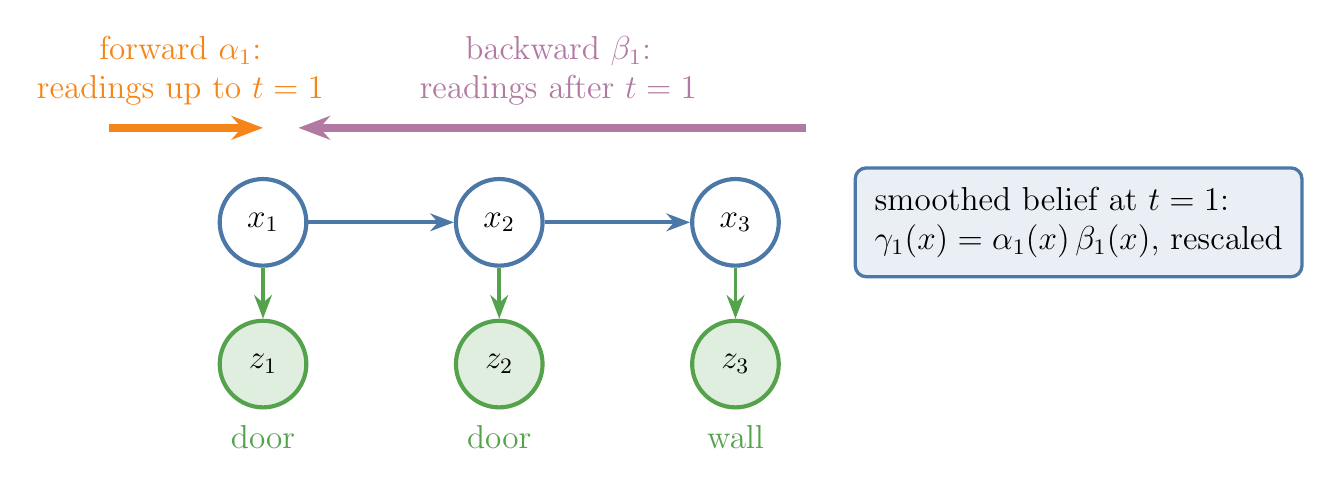
\begin{tikzpicture}[x=3cm, y=1cm, every node/.append style={font=\large},
    hid/.style={circle, draw=cblue, line width=1.5pt, minimum size=1.1cm, fill=white},
    obs/.style={circle, draw=cgreen, line width=1.5pt, minimum size=1.1cm, fill=cgreen!18}]
  \foreach \t/\z in {1/door, 2/door, 3/wall} {
    \node[hid] (x\t) at (\t,0) {$x_\t$};
    \node[obs] (z\t) at (\t,-1.8) {$z_\t$};
    \node[cgreen, below=2pt] at (z\t.south) {\z};
    \draw[arrow, draw=cgreen] (x\t) -- (z\t);
  }
  \draw[arrow, draw=cblue] (x1) -- (x2);
  \draw[arrow, draw=cblue] (x2) -- (x3);
  \draw[-{Stealth[length=4mm]}, corange, line width=3pt] (0.35,1.2) -- (1.0,1.2);
  \node[corange, align=center, anchor=south] at (0.65,1.35) {forward $\alpha_1$:\\readings up to $t = 1$};
  \draw[-{Stealth[length=4mm]}, cpurple, line width=3pt] (3.3,1.2) -- (1.15,1.2);
  \node[cpurple, align=center, anchor=south] at (2.25,1.35) {backward $\beta_1$:\\readings after $t = 1$};
  \node[box=cblue, anchor=west, align=left] at (3.5,0) {smoothed belief at $t = 1$:\\$\gamma_1(x) = \alpha_1(x)\,\beta_1(x)$, rescaled};
\end{tikzpicture}
\end{document}
